The second examples is the The second-order moving average (MA2),
which is internally implemented in the ELFI package. This example is
chosen to confirm that the ROMC implementation works well under a
general model, not implemented by us.

\subsubsection*{Problem definition}

The second-order moving average (MA2) is a common model used for
univariate time series analysis. The observation at time $t$ is given by:

\begin{gather} \label{eq:ma2}
y_t = w_t + \theta_1 w_{t-1} + \theta_2 w_{t-2}\\
\theta_1, \theta_2 \in \R, \quad  w_{k, k \in \mathbb{Z}} \sim \mathcal{N}(0,1)
\end{gather}

As we can notice, $w_{k, k \in \mathbb{Z}} \sim \mathcal{N}(0,1)$
represents an independent and identically distributed white noise and
$\theta_1, \theta_2$ the dependence from the previous
observations. The number of consecutive observations $T$ is a
hyper-parameter of the model; in our case we will set
$T=100$. Computing the likelihood of the MA2 model is generally
difficult, due to the unobserved noise variables
$w_t, w_{t-1}, w_{t-2}$, and it becomes intractable in cases where $T$
is large. On the other hand, generating an MA2 time-series is pretty
easy and efficient using a simulator; this makes the likelihood-free
inference methods quite convenient for the particular model.

At our example, we use the prior as defined by \autocite{Marin2012}
for guaranteeing that the inference problem is identifiable i.e.\
loosely speaking, the likelihood will have just one mode. The
multivariate prior, which is given in the equation
\eqref{eq:ma2_prior}, follows a triangular shape as ploted in figure
\ref{fig:ma2_1}.

\begin{equation} \label{eq:ma2_prior}
p(\thetab) = p(\theta_1)p(\theta_2|\theta_1)
= \mathcal{U}(\theta_1;-2,2)\mathcal{U}(\theta_2;\theta_1-1, \theta_1+1)
\end{equation}

\begin{figure}[h]
    \begin{center}
      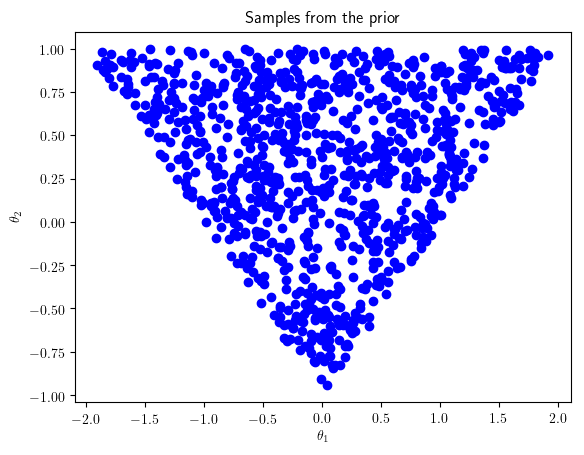
\includegraphics[width=0.48\textwidth]{./Thesis/images/chapter4/mae2_prior_samples.png}
    \end{center}
  \caption{Prior distribution as define by Marin et al.\ \autocite{Marin2012}.}
  \label{fig:ma2_1}
\end{figure}

The vector $\yb_0 = (y_1, \ldots, y_{100})$, used as the observation,
is generated with $\thetab=(0.6, 0.2)$.


\subsubsection*{Perform the inference}

As in the previous example, we perform the inference using both
optimisation versions, the gradient-based and the Bayesian
optimisation; in this way, we compare the results obtained in each
step. Since in this example it is impossible to obtain ground-truth
information, we use the samples obtained with Rejection ABC sampling
for comparison.

In figure \ref{fig:ma2_2} we observe that in most cases the optimal
distance $d_i^*$ is close to zero in both optimisation approaches.

In figure \ref{mae2_5}, we have chosen three different optimisation
examples for illustrating three different cases. In the first case,
both optimisation schemes lead to the same bounding box. In the second
case, the bounding box has similar shape, different size and it is
shifted along the $\theta_1$ axis. Finally, in the third case, both
the bounding box and the optimal point are completely different. This
leads conclusion, that although fitting a surrogate model has
important computational advantages, there is no guarantee that it will
reproduce the local region around the optimal point with
accuracy. This approximation error leads sometimes to the construction
of quite different proposal regions, which in turn, explains the small
differences in the histogram of the marginal distributions presented
in figure \ref{fig:ma2_3} and in the approximate posteriors in figure
\ref{fig:ma2_4}.

The histograms of the marginal posteriors are similar between all
approaches, as shown in figure \ref{fig:ma2_3}. In the table
\ref{tab:ma2} we present the empirical mean $\mu$ and standard
deviation $\sigma$ in all cases. We observe that there is a general
agreement between the approaches, which verifies that the ROMC
implementation provides sensible results. Finally, in figure
\ref{fig:ma2_4} we provide the ROMC approximate posteriors using
gradients and Bayesian optimisation; as confirmed by the statistics in
\ref{tab:ma2}, both posteriors have a single mode, located at the same
point, with a larger variance observed in the Bayesian Optimisation
case.

\begin{center} \label{tab:ma2}
\begin{tabular}{ c|c|c|c|c }
\hline
& $\mu_{\theta_1}$ & $\sigma_{\theta_1}$ & $\mu_{\theta_2}$ & $\sigma_{\theta_2}$ \\
\hline \hline
Rejection ABC & 0.516 & 0.142 & 0.07 & 0.172 \\
\hline
ROMC (gradient-based) & 0.495 & 0.136 & 0.048 & 0.178 \\
\hline
ROMC (Bayesian optimisation) & 0.510 & 0.156 & 0.108 & 0.183 \\
\hline
\end{tabular}
\end{center}

\begin{figure}[h]
    \begin{center}
      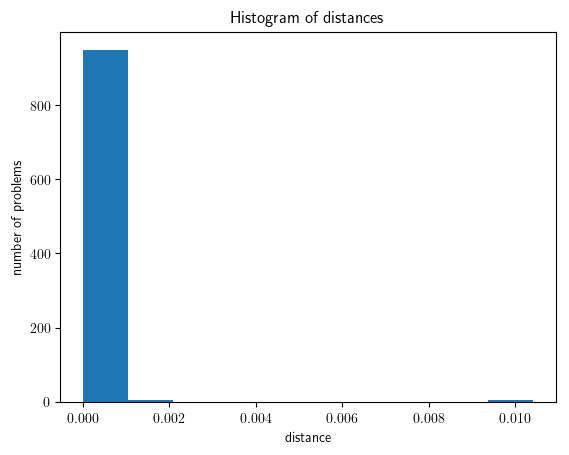
\includegraphics[width=0.48\textwidth]{./Thesis/images/chapter4/ma2_distance_hist.png}
      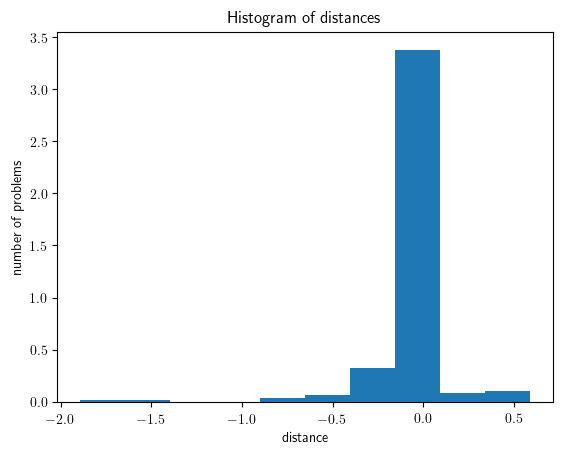
\includegraphics[width=0.48\textwidth]{./Thesis/images/chapter4/ma2_distance_hist_bo.png}
    \end{center}
  \caption{Histogram of distances $d_{i, i \in {1, \ldots, n_1}}^*$. The left graph corresponds to the gradient-based approach and the right one to the Bayesian optimisation approach.}
  \label{fig:ma2_2}
\end{figure}

\begin{figure}[h]
    \begin{center}
      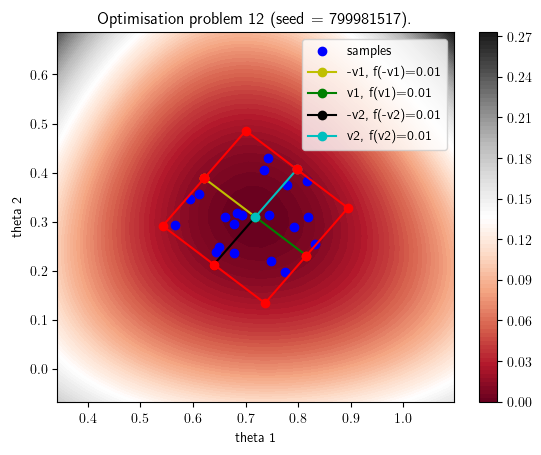
\includegraphics[width=0.48\textwidth]{./Thesis/images/chapter4/ma2_region_1.png}
      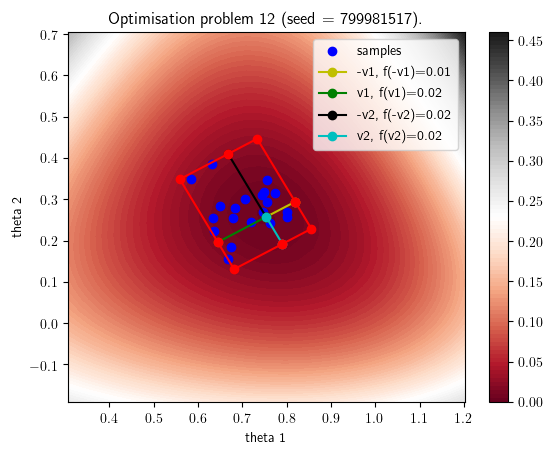
\includegraphics[width=0.48\textwidth]{./Thesis/images/chapter4/ma2_region_1_bo.png}\\
      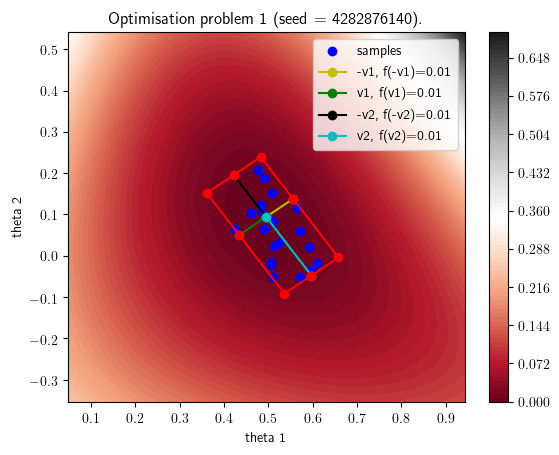
\includegraphics[width=0.48\textwidth]{./Thesis/images/chapter4/ma2_region_2.png}
      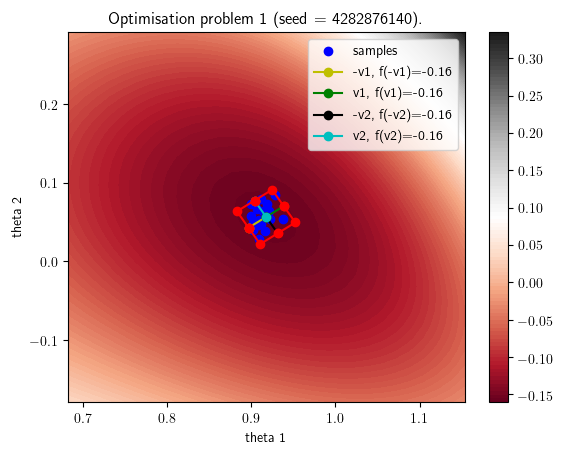
\includegraphics[width=0.48\textwidth]{./Thesis/images/chapter4/ma2_region_2_bo.png}\\
      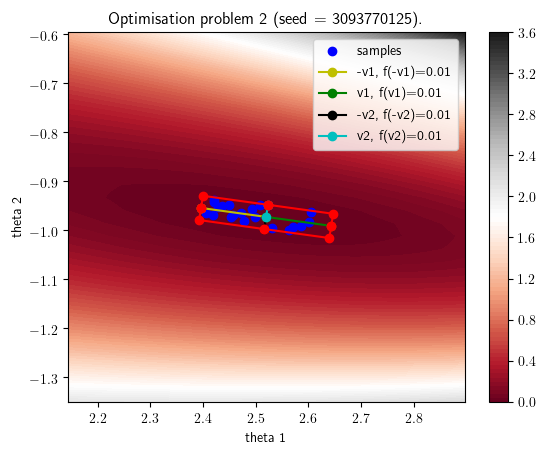
\includegraphics[width=0.48\textwidth]{./Thesis/images/chapter4/ma2_region_3.png}
      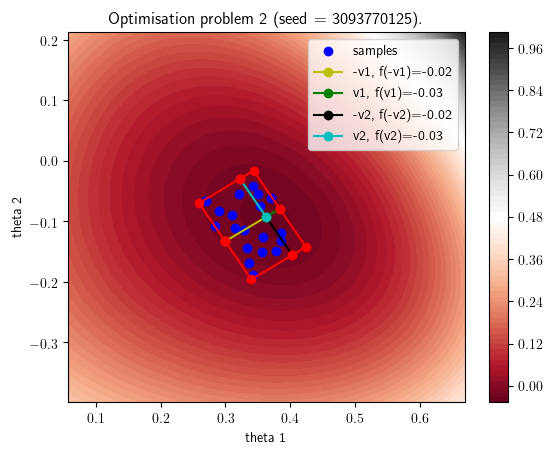
\includegraphics[width=0.48\textwidth]{./Thesis/images/chapter4/ma2_region_3_bo.png}
    \end{center}
  \caption{Visualisation of the acceptance region in 3 different optimisation problems. Each row illustrates a different optimisation problem, the left column corresponds to the gradient-based approach and the right column to the Bayesian optimisation approach. The examples have been chosen to illustrate three different cases; in the first case, both optimisation schemes lead to similar optimal point and bounding box, in the second case the bounding box is similar in shape but a little bit shifted to the right relatively to the gradient-based approach and in the third case, both the optimal point and the bounding box is completely different.}
  \label{fig:ma2_5}
\end{figure}


\begin{figure}[h]
    \begin{center}
      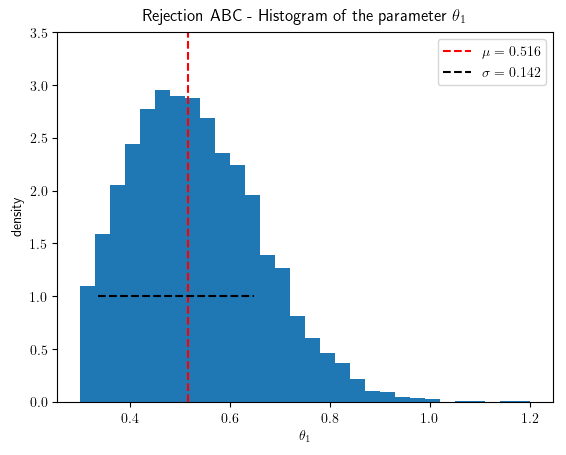
\includegraphics[width=0.48\textwidth]{./Thesis/images/chapter4/mae2_hist_t1_rejection.png}
      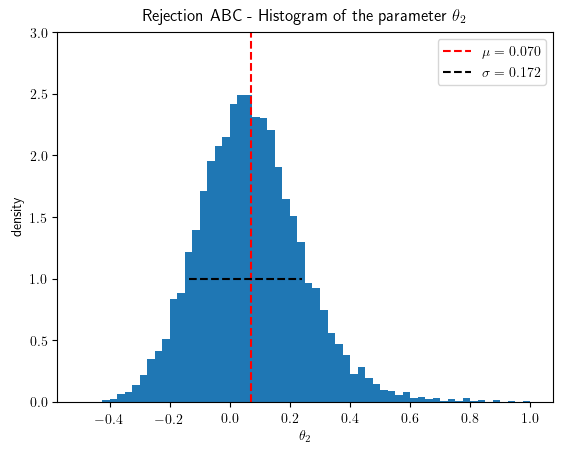
\includegraphics[width=0.48\textwidth]{./Thesis/images/chapter4/mae2_hist_t2_rejection.png}\\
      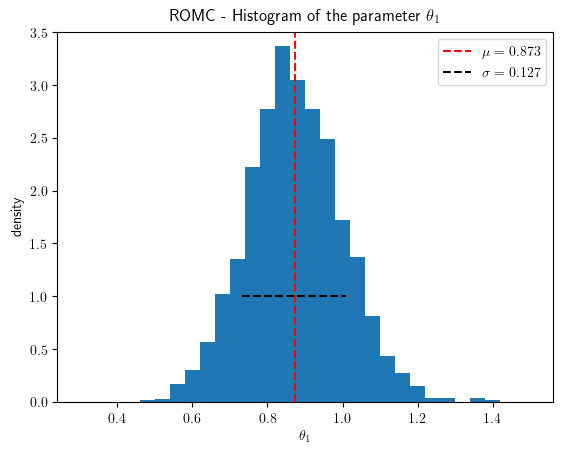
\includegraphics[width=0.48\textwidth]{./Thesis/images/chapter4/mae2_hist_t1_romc.png}
      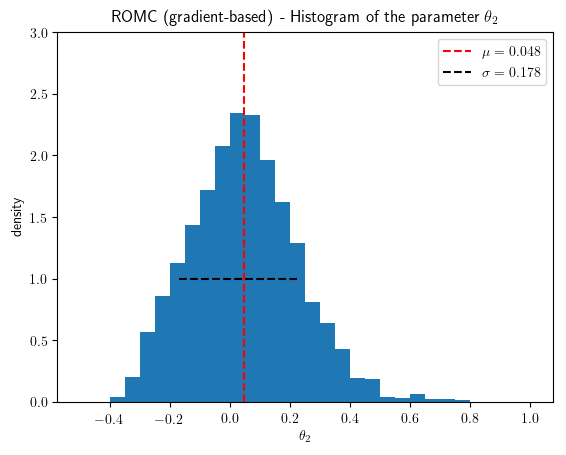
\includegraphics[width=0.48\textwidth]{./Thesis/images/chapter4/mae2_hist_t2_romc.png}\\
      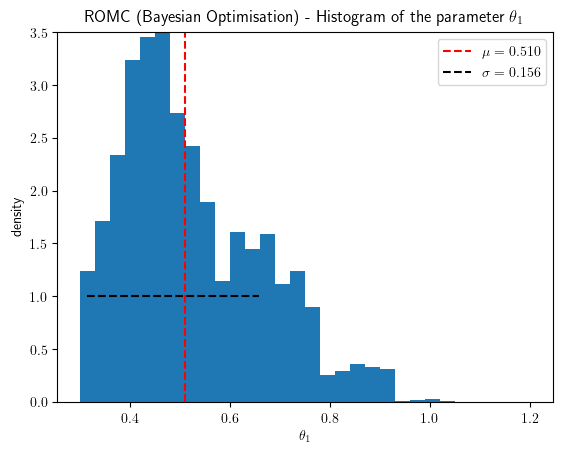
\includegraphics[width=0.48\textwidth]{./Thesis/images/chapter4/mae2_hist_t1_romc_bo.png}
      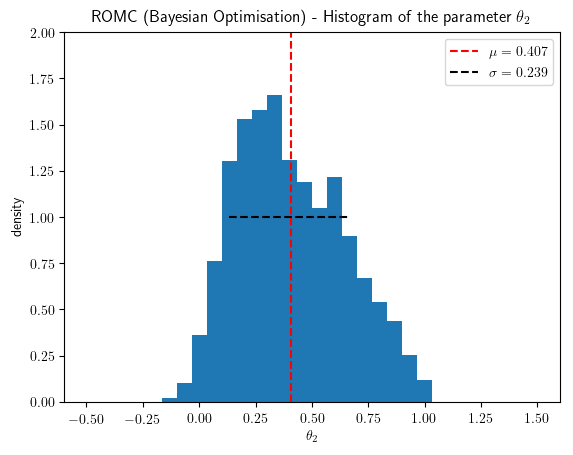
\includegraphics[width=0.48\textwidth]{./Thesis/images/chapter4/mae2_hist_t2_romc_bo.png}\\
    \end{center}
  \caption{Histogram of the marginal distribution for three different inference approaches; (a) in the first row, the approximate posterior samples are obtained using Rejection ABC sampling (b) in the second row, using ROMC sampling with gradient-based approach and (c) in the third row, using ROMC sampling with Bayesian optimisation approach. The vertical (red) line represents the samples mean $\mu$ and the horizontal (black) the standard deviation $\sigma$.}
  \label{fig:ma2_3}
\end{figure}


\begin{figure}[h]
    \begin{center}
      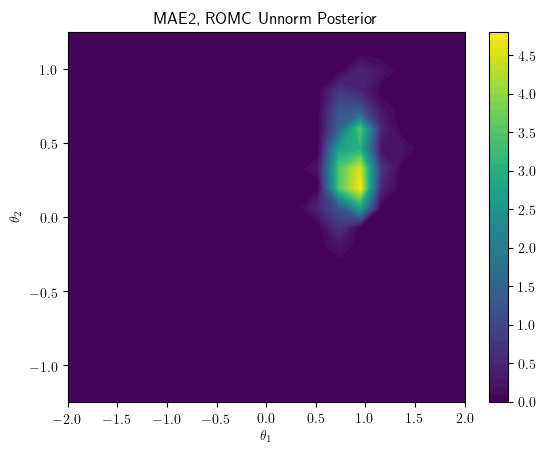
\includegraphics[width=0.48\textwidth]{./Thesis/images/chapter4/mae2_romc_posterior.png}
      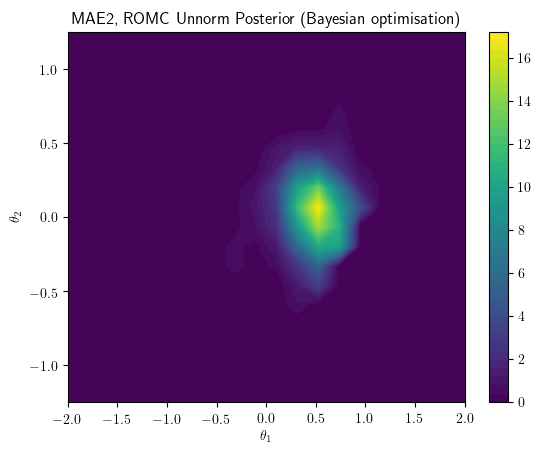
\includegraphics[width=0.48\textwidth]{./Thesis/images/chapter4/mae2_romc_posterior_bo.png}
    \end{center}
  \caption{ROMC approximate posteriors using gradient-based approach (left) and Bayesian optimisation approach (right).}
  \label{fig:ma2_4}
\end{figure}

